% preamble-exam-zh.tex — 极简讲解页共享 preamble
% 目标：复刻「题目独立、提示轻框、路线箭头、主体双栏、答案轻收束」的讲义风格。

\documentclass{exam-zh}

% ---------- 基础配置 ----------
\examsetup{
  page/size = a4paper,
  page/show-head = false,
  page/show-foot = false,
  sealline/show = false,
  font = none,
  math-font = none,
}

% ---------- 包 ----------
\usepackage{geometry}
\geometry{top=10mm,bottom=14mm,left=12mm,right=10mm}
\AtBeginDocument{\newgeometry{top=10mm,bottom=14mm,left=12mm,right=10mm}}

\usepackage{xcolor}
\usepackage{needspace}
\usepackage{enumitem}
\usepackage{array}
\usepackage{tabularx}
\usepackage{tcolorbox}
\tcbuselibrary{skins,breakable}
\usepackage{paracol}
\usepackage{graphicx}

% ---------- 打印/屏幕颜色切换 ----------
% 用法：\documentclass[monochrome]{exam-zh} 可降级为灰度。
% 注意：不要使用 \if@xxx 放在 makeatother 外部；这里改成普通条件名。
\newif\ifeduprintcolor
\eduprintcolortrue
\makeatletter
\@ifclasswith{exam-zh}{monochrome}{\eduprintcolorfalse}{}
\makeatother

% ---------- 语义颜色 ----------
\ifeduprintcolor
  \definecolor{edu-blue}{RGB}{31,62,126}
  \definecolor{edu-blue-soft}{RGB}{232,238,250}
  \definecolor{edu-blue-bg}{RGB}{248,250,254}
  \definecolor{edu-ink}{RGB}{30,35,45}
  \definecolor{edu-muted}{RGB}{118,124,136}
  \definecolor{edu-line}{RGB}{209,218,235}
  \definecolor{edu-soft-bg}{RGB}{250,251,253}
  \definecolor{edu-red}{RGB}{168,58,58}
  \definecolor{edu-red-bg}{RGB}{255,247,245}
\else
  \definecolor{edu-blue}{gray}{0.15}
  \definecolor{edu-blue-soft}{gray}{0.90}
  \definecolor{edu-blue-bg}{gray}{0.98}
  \definecolor{edu-ink}{gray}{0.10}
  \definecolor{edu-muted}{gray}{0.45}
  \definecolor{edu-line}{gray}{0.82}
  \definecolor{edu-soft-bg}{gray}{0.97}
  \definecolor{edu-red}{gray}{0.28}
  \definecolor{edu-red-bg}{gray}{0.97}
\fi
\colorlet{edu-diagram-muted}{edu-muted}

% ---------- 全局排版 ----------
\setlength{\parindent}{0pt}
\setlength{\parskip}{0pt}
\linespread{1.16}
\renewcommand{\arraystretch}{1.15}

% ctex 通常提供 \kaishu；这里用它做教师旁白感。
\newcommand{\edukai}{\kaishu}

% ---------- 顶部元信息 ----------
\newcommand{\eduTopBar}[2]{%
  \noindent
  \begin{tabularx}{\linewidth}{@{}Xr@{}}
    {\color{edu-blue}\bfseries #1} &
    {\color{edu-blue}\bfseries #2}
  \end{tabularx}
  \vspace{8mm}
}

% ---------- 轻标题体系 ----------
% 只有真正的大结构才用它；不要给提示/路线滥用标题。
\newcommand{\eduSectionTitle}[1]{%
  \needspace{5\baselineskip}%
  \vspace{2mm}
  {\color{edu-blue}\bfseries\large #1}\par
  \vspace{3mm}
}

\newcommand{\eduSubTitle}[1]{%
  \needspace{4\baselineskip}%
  \vspace{1mm}
  {\color{edu-blue}\bfseries #1}\par
  \vspace{1mm}
}

% ---------- 小问题干：复用 exam (1)(2)(3) 格式 ----------
\newenvironment{eduSubQuestionItem}[1]{%
  \needspace{4\baselineskip}%
  \vspace{2mm}
  \par\noindent
  \hangindent=8mm\hangafter=1
  {\color{edu-blue}\bfseries #1}\enspace
  \begingroup
  \color{edu-ink}
}{%
  \endgroup
  \par
  \vspace{3mm}
}

% ---------- 辅助信息条（解题流程/关键想法/思考）楷体 ----------
\newenvironment{eduAuxItem}[1]{%
  \needspace{4\baselineskip}%
  \vspace{2mm}
  \par\noindent
  \hangindent=8mm\hangafter=1
  {\color{edu-blue}\edukai $\triangleright$~#1}\enspace
  \begingroup
  \color{edu-ink}
  \edukai
}{%
  \endgroup
  \par
  \vspace{4mm}
}

\newcommand{\eduColumnTitle}[2]{%
  {\color{edu-blue}\bfseries #1\hspace{1.5mm}#2}\par
  \vspace{2.5mm}
}

% ---------- 图标：不用外部 icon 字体，保证可移植 ----------
\newcommand{\eduIconBulb}{\(\circ\)}
\newcommand{\eduIconBook}{\(\square\)}
\newcommand{\eduIconCheck}{\(\checkmark\)}
\newcommand{\eduIconPin}{\(\diamond\)}
\newcommand{\eduIconNote}{\(\triangleright\)}

% ---------- 题目区 ----------
% 题目区是页面入口：弱标签 + 一条长蓝线 + 大题干。
\newenvironment{eduProblemBlock}[1][题目]{%
  \needspace{8\baselineskip}
  {\small\color{edu-muted}#1}\par
  \vspace{1.5mm}
  {\color{edu-blue}\hrule height 0.55pt}
  \vspace{4.5mm}
  \begingroup
  \color{edu-ink}
  \large
  \setlength{\parskip}{2.2mm}
  \linespread{1.20}\selectfont
}{%
  \par
  \endgroup
  \vspace{6mm}
}

\newenvironment{eduSubQuestions}{%
  \begin{enumerate}[
    label=(\arabic*),
    leftmargin=8mm,
    itemsep=2.0mm,
    topsep=2.0mm,
    parsep=0pt
  ]
}{%
  \end{enumerate}
}

% ---------- 读题提示：轻框，不做同级标题 ----------
\newtcolorbox{eduReadTipBox}{
  enhanced,
  breakable,
  colback=white,
  colframe=edu-blue!45,
  boxrule=0.45pt,
  arc=1.6mm,
  left=10mm,
  right=4mm,
  top=5mm,
  bottom=5mm,
  before skip=1mm,
  after skip=7mm,
  fontupper=\edukai\normalsize,
  colupper=edu-ink,
  overlay={
    \node[anchor=north west, text=edu-blue] at ([xshift=3.2mm,yshift=-3.2mm]frame.north west)
    {\small\eduIconNote};
  }
}

\newenvironment{eduTipList}{%
  \begin{itemize}[
    label=\textbullet,
    leftmargin=5mm,
    itemsep=1.2mm,
    topsep=0pt,
    parsep=0pt
  ]
}{%
  \end{itemize}
}

% ---------- 解题路线：虚线框 + 文字箭头 ----------
\newenvironment{eduRouteFlow}{%
  \needspace{4\baselineskip}%
  \vspace{1mm}
  \begin{center}
  \normalsize
}{%
  \end{center}
  \vspace{7mm}
}
\newcommand{\eduRouteStep}[1]{%
  {\color{edu-ink}#1}%
}
\newcommand{\eduRouteArrow}{%
  \;$\boldsymbol{\to}$\;%
}

% ---------- 主体讲解：使用 paracol 实现跨页自适应双栏 ----------
\newenvironment{eduDualExplain}{%
  \needspace{6\baselineskip}% 防止标题孤行
  \columnratio{0.26, 0.74}%
  \setlength{\columnsep}{8mm}%
  \columnseprule=0.45pt%
  \colseprulecolor{edu-blue}%
  \begin{paracol}{2}% 开启双栏
}{%
  \end{paracol}% 结束双栏
  \vspace{5mm}
}

\newenvironment{eduExplainLeft}{%
  \setlength{\linewidth}{\columnwidth}%
  \hsize=\columnwidth
  \normalsize\color{edu-ink}%
}{%
  \switchcolumn
}

\newcommand{\eduColumnDivider}{}

\newenvironment{eduExplainRight}{%
  \setlength{\linewidth}{\columnwidth}%
  \hsize=\columnwidth
  \normalsize\color{edu-ink}%
}{%
}

\newtcolorbox{eduSideHintBox}[1]{
  enhanced,
  breakable,
  colback=edu-blue-bg,
  colframe=edu-line,
  boxrule=0.35pt,
  borderline west={1.5pt}{0pt}{edu-blue},
  arc=0.8mm,
  left=2.4mm,
  right=2.4mm,
  top=2mm,
  bottom=2mm,
  before skip=1mm,
  after skip=1.5mm,
  title={\color{edu-blue}\bfseries\small #1},
  coltitle=edu-blue,
  attach title to upper={\par\vspace{0.7mm}},
  fontupper=\small
}

\newtcolorbox{eduSideMistakeBox}[1]{
  enhanced,
  breakable,
  colback=edu-red-bg,
  colframe=edu-red!35,
  boxrule=0.35pt,
  borderline west={1.5pt}{0pt}{edu-red},
  arc=0.8mm,
  left=2.4mm,
  right=2.4mm,
  top=2mm,
  bottom=2mm,
  before skip=1mm,
  after skip=1.5mm,
  title={\color{edu-red}\bfseries\small #1},
  coltitle=edu-red,
  attach title to upper={\par\vspace{0.7mm}},
  fontupper=\small
}

\newtcolorbox{eduSideNoteBox}[1]{
  enhanced,
  breakable,
  colback=edu-soft-bg,
  colframe=edu-line,
  boxrule=0.35pt,
  borderline west={1.5pt}{0pt}{edu-muted},
  arc=0.8mm,
  left=2.4mm,
  right=2.4mm,
  top=2mm,
  bottom=2mm,
  before skip=1mm,
  after skip=1.5mm,
  title={\color{edu-muted}\bfseries\small #1},
  coltitle=edu-muted,
  attach title to upper={\par\vspace{0.7mm}},
  fontupper=\small
}

\newcommand{\eduSideHint}[2]{%
  \begin{eduSideHintBox}{#1}#2\end{eduSideHintBox}%
}
\newcommand{\eduSideMistake}[2]{%
  \begin{eduSideMistakeBox}{#1}#2\end{eduSideMistakeBox}%
}
\newcommand{\eduSideNote}[2]{%
  \begin{eduSideNoteBox}{#1}#2\end{eduSideNoteBox}%
}

\newcommand{\eduExplainStep}[3]{%
  \needspace{3\baselineskip}%
  \vspace{1.2mm}%
  {\color{edu-blue}\bfseries step#1.\enspace #2}\par
  \vspace{0.8mm}%
  \begingroup
  \color{edu-ink}#3\par
  \endgroup
  \vspace{2.2mm}%
}

\newenvironment{eduNumberList}{%
  \begin{enumerate}[
    label=\arabic*.,
    leftmargin=6mm,
    itemsep=4.8mm,
    topsep=0pt,
    parsep=0pt
  ]
}{%
  \end{enumerate}
}

\newenvironment{eduBulletList}{%
  \begin{itemize}[
    label=\textbullet,
    leftmargin=5mm,
    itemsep=1.2mm,
    topsep=0pt,
    parsep=0pt
  ]
}{%
  \end{itemize}
}

% ---------- 底部双栏：答案 + 方法提醒 ----------
\newenvironment{eduBottomGrid}{%
  \columnratio{0.32, 0.68}%
  \setlength{\columnsep}{11mm}%
  \columnseprule=0pt%
  \begin{paracol}{2}%
}{%
  \end{paracol}%
}

\newenvironment{eduSummaryLeft}{%
}{%
}

\newcommand{\eduSummaryDivider}{%
  \switchcolumn
}

\newenvironment{eduSummaryRight}{%
}{%
}

% ---------- 答案/方法提醒：轻量收束 ----------
\newtcolorbox{eduSummaryBlock}[2]{
  enhanced,
  breakable,
  colback=edu-blue-bg,
  colframe=edu-line,
  boxrule=0.45pt,
  arc=1.2mm,
  left=3.5mm,
  right=3.5mm,
  top=3mm,
  bottom=3mm,
  before skip=1mm,
  after skip=2.5mm,
  title={\color{edu-blue}\bfseries #1\hspace{1.5mm}#2},
  coltitle=edu-blue,
  attach title to upper={\par\vspace{1.5mm}},
  fontupper=\normalsize
}

% ---------- 例题单栏解答卡片 ----------
\newtcolorbox{eduSolutionBox}[1]{
  enhanced,
  breakable,
  colback=white,
  colframe=edu-blue!40,
  boxrule=0.55pt,
  arc=1.2mm,
  left=4mm,
  right=4mm,
  top=3.5mm,
  bottom=3.5mm,
  before skip=2mm,
  after skip=3mm,
  title={\color{edu-blue}\bfseries \eduIconBook\hspace{1.5mm}#1},
  coltitle=edu-blue,
  attach title to upper={\par\vspace{1.5mm}},
  fontupper=\normalsize
}

% ---------- 变式训练：完整题目 + 学生留白 ----------
\newtcolorbox{eduVariationTraining}[1]{
  enhanced,
  breakable,
  colback=white,
  colframe=edu-blue!45,
  boxrule=0.5pt,
  borderline west={1.8pt}{0pt}{edu-blue},
  arc=1.2mm,
  left=4mm,
  right=4mm,
  top=3.2mm,
  bottom=3.2mm,
  before skip=2mm,
  after skip=4mm,
  title={\color{edu-blue}\bfseries #1},
  coltitle=edu-blue,
  attach title to upper={\par\vspace{1.8mm}},
  fontupper=\normalsize,
  colupper=edu-ink
}

\newenvironment{eduPlainList}{%
  \begin{enumerate}[
    label=(\arabic*),
    leftmargin=7mm,
    itemsep=1.2mm,
    topsep=0pt,
    parsep=0pt
  ]
}{%
  \end{enumerate}
}

% ---------- 兼容旧 block 的轻量盒子 ----------
\newtcolorbox{eduSoftBox}{
  enhanced,
  breakable,
  colback=edu-soft-bg,
  colframe=edu-line,
  boxrule=0.35pt,
  arc=1mm,
  left=3mm,
  right=3mm,
  top=2mm,
  bottom=2mm,
  before skip=1mm,
  after skip=2mm,
  fontupper=\small
}

\newtcolorbox{eduMistakeBox}{
  enhanced,
  breakable,
  colback=edu-red-bg,
  colframe=edu-red!40,
  boxrule=0.35pt,
  arc=1mm,
  left=3mm,
  right=3mm,
  top=2.5mm,
  bottom=2.5mm,
  before skip=1mm,
  after skip=2mm,
  fontupper=\normalsize
}

\newtcolorbox{eduLegacySolution}{
  enhanced,
  breakable,
  colback=edu-soft-bg,
  colframe=edu-line,
  boxrule=0.35pt,
  arc=1mm,
  left=3mm,
  right=3mm,
  top=2mm,
  bottom=2mm,
  before skip=-2mm,
  after skip=4mm,
  fontupper=\small
}

\newtcolorbox{eduTeacherNote}{
  enhanced,
  breakable,
  colback=edu-soft-bg,
  colframe=edu-line,
  boxrule=0pt,
  borderline west={1.5pt}{0pt}{edu-muted},
  left=2.5mm,
  right=2.5mm,
  top=2mm,
  bottom=2mm,
  before skip=1mm,
  after skip=2mm,
  fontupper=\footnotesize,
  colupper=edu-muted
}

% ---------- 答题区 ----------
\newcommand{\answerarea}[1][40mm]{%
  \vspace{3mm}%
  \begin{tcolorbox}[
    enhanced,
    breakable,
    colback=white,
    colframe=edu-line,
    boxrule=0.55pt,
    arc=0.8mm,
    height=#1,
    valign=top,
  ]
  \end{tcolorbox}%
}

\newcommand{\diagramcolfigure}[3]{%
  \begin{minipage}[t]{#2}
    \vspace{0pt}\centering
    \includegraphics[width=\linewidth]{\detokenize{#1}}
    \if\relax\detokenize{#3}\relax\else
      \par\vspace{1mm}{\scriptsize\color{edu-diagram-muted}#3}
    \fi
  \end{minipage}%
}

\newcommand{\diagramrowitem}[4]{%
  \begin{minipage}[t]{#2}
    \vspace{0pt}\centering
    \includegraphics[width=\linewidth]{\detokenize{#1}}
    \if\relax\detokenize{#3}\relax\else
      \par\vspace{1mm}{\scriptsize\bfseries #3}
    \fi
    \if\relax\detokenize{#4}\relax\else
      \par\vspace{0.5mm}{\scriptsize\color{edu-diagram-muted}#4}
    \fi
  \end{minipage}%
}

\newcommand{\answerareawithdiagramcol}[4]{%
  \vspace{3mm}%
  \begin{tcolorbox}[
    enhanced,
    breakable,
    colback=white,
    colframe=edu-line,
    boxrule=0.55pt,
    arc=0.8mm,
    height=#1,
    valign=top,
  ]
  \begin{minipage}[t]{\dimexpr\linewidth-#3-6mm\relax}
    \vspace{0pt}
  \end{minipage}\hfill
  \diagramcolfigure{#2}{#3}{#4}
  \end{tcolorbox}%
}

\newcommand{\answerareawithdiagram}[4]{%
  \answerareawithdiagramcol{#1}{#2}{#3}{#4}%
}

\examsetup{
  question/show-answer = true,
  fillin/show-answer = true,
  solution/show-solution = show-stay,
}

\begin{document}

\eduSectionTitle{模型：反比例函数中的面积不变量}


\begin{eduSolutionBox}{核心结论：矩形是 $|k|$，三角形是 $|k|/2$}
  \begingroup
  \setlength{\parskip}{2.5mm}
若 $A(x,y)$ 在 $y=\dfrac{k}{x}$ 上，则 $xy=k$。\par
由 $A$ 向两坐标轴作垂线，围成的矩形面积为 $|x|\cdot |y|=|k|$。\par
与坐标轴和原点围成的直角三角形面积为 $\dfrac12|x|\cdot |y|=\dfrac{|k|}{2}$。\par
面积只能先确定 $|k|$，$k$ 的符号要看象限或增减性。\par
  \endgroup
\end{eduSolutionBox}




\begin{eduProblemBlock}[例题 1]
如图，点 $A$ 在反比例函数 $y=\dfrac{k}{x}$ 的图像上，过点 $A$ 分别向坐标轴作垂线。若围成的矩形面积为 $12$，且图像在第二、四象限，求 $k$。
\begin{center}
\begin{tikzpicture}[scale=0.45,>=latex]
  \draw[->] (-4.8,0)--(4.8,0) node[right]{$x$};
  \draw[->] (0,-3.8)--(0,3.8) node[above]{$y$};
  \node[below right] at (0,0){$O$};
  \draw[smooth,domain=-4.5:-0.8,samples=80] plot(\x,{-4/\x});
  \draw[smooth,domain=0.8:4.5,samples=80] plot(\x,{-4/\x});
  \coordinate (A) at (-3,1.33);
  \draw[dashed] (A)--(-3,0) node[below]{$M$};
  \draw[dashed] (A)--(0,1.33) node[right]{$N$};
  \draw (-3,0)--(0,0)--(0,1.33)--(A)--cycle;
  \fill (A) circle(2pt) node[above left]{$A$};
\end{tikzpicture}
\end{center}

\end{eduProblemBlock}





\begin{eduAuxItem}{思路导航}
矩形面积对应 $|k|$$\;\to\;$用象限确定符号\end{eduAuxItem}




\begin{eduSubQuestionItem}{例题 1}
求反比例函数系数 $k$。\end{eduSubQuestionItem}

\begin{eduDualExplain}
  \begin{eduExplainLeft}
    \eduColumnTitle{\eduIconBulb}{小贴士}
        \eduSideHint{面积没有符号}{先得到 $|k|$，再根据图像所在象限判断正负。}
  \end{eduExplainLeft}

  \begin{eduExplainRight}
    \eduColumnTitle{\eduIconBook}{解答}
      \eduExplainStep{1}{矩形面积对应 $|k|$}{围成的矩形面积为 $|k|$，所以 $|k|=12$。}
      \eduExplainStep{2}{用象限确定符号}{图像在第二、四象限，所以 $k<0$。因此 $k=-12$。}
  \end{eduExplainRight}
\end{eduDualExplain}




\begin{eduProblemBlock}[例题 2]
如图，点 $A(x,y)$ 在反比例函数 $y=\dfrac{k}{x}$ 上，过 $A$ 向 $x$ 轴作垂线，垂足为 $M$。点 $C(0,4)$ 在 $y$ 轴上。若 $\triangle AMC$ 的面积为 $10$，且点 $A$ 在第四象限，求 $k$。
\begin{center}
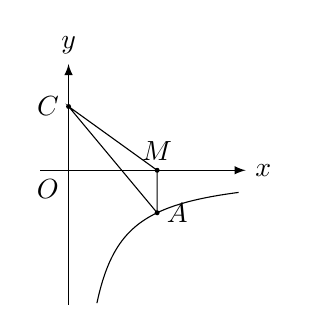
\begin{tikzpicture}[scale=0.45,>=latex]
  \draw[->] (-0.8,0)--(5,0) node[right]{$x$};
  \draw[->] (0,-3.8)--(0,3) node[above]{$y$};
  \node[below left] at (0,0){$O$};
  \draw[smooth,domain=0.8:4.8,samples=80] plot(\x,{-3/\x});
  \coordinate (A) at (2.5,-1.2);
  \coordinate (M) at (2.5,0);
  \coordinate (C) at (0,1.8);
  \draw (A)--(M)--(C)--cycle;
  \fill (A) circle(2pt) node[right]{$A$};
  \fill (M) circle(2pt) node[above]{$M$};
  \fill (C) circle(2pt) node[left]{$C$};
\end{tikzpicture}
\end{center}

\end{eduProblemBlock}





\begin{eduAuxItem}{思路导航}
找底和高$\;\to\;$面积回到 $|k|/2$$\;\to\;$用象限确定符号\end{eduAuxItem}




\begin{eduSubQuestionItem}{例题 2}
点 $C$ 在坐标轴上时，用面积求 $k$。\end{eduSubQuestionItem}

\begin{eduDualExplain}
  \begin{eduExplainLeft}
    \eduColumnTitle{\eduIconBulb}{小贴士}
        \eduSideMistake{别把 C 的坐标直接当高}{高是点到直线 $AM$ 的距离，不是 $C$ 的纵坐标。}
  \end{eduExplainLeft}

  \begin{eduExplainRight}
    \eduColumnTitle{\eduIconBook}{解答}
      \eduExplainStep{1}{找底和高}{$AM=|y|$，点 $C$ 到直线 $AM$ 的距离为 $|x|$。}
      \eduExplainStep{2}{面积回到 $|k|/2$}{$S_{\triangle AMC}=\dfrac12|x|\cdot |y|=\dfrac{|k|}{2}$。由 $\dfrac{|k|}{2}=10$ 得 $|k|=20$。}
      \eduExplainStep{3}{用象限确定符号}{$A$ 在第四象限，$xy<0$，所以 $k=-20$。}
  \end{eduExplainRight}
\end{eduDualExplain}




\begin{eduProblemBlock}[例题 3]
如图，点 $A$ 在反比例函数 $y=\dfrac{k}{x}$ 当 $x<0$ 时的图像上，过点 $A$ 作 $AB\perp x$ 轴，垂足为 $D$，且 $D$ 是线段 $AB$ 的中点。点 $C$ 在 $y$ 轴上，若 $\triangle ABC$ 的面积为 $9$，求 $k$。
\begin{center}
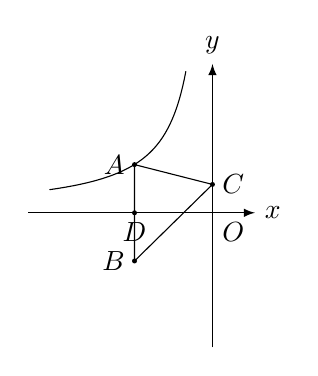
\begin{tikzpicture}[scale=0.45,>=latex]
  \draw[->] (-5.2,0)--(1.2,0) node[right]{$x$};
  \draw[->] (0,-3.8)--(0,4.2) node[above]{$y$};
  \node[below right] at (0,0){$O$};
  \draw[smooth,domain=-4.6:-0.75,samples=80] plot(\x,{-3/\x});
  \coordinate (A) at (-2.2,1.36);
  \coordinate (D) at (-2.2,0);
  \coordinate (B) at (-2.2,-1.36);
  \coordinate (C) at (0,0.8);
  \draw (A)--(B)--(C)--cycle;
  \draw[dashed] (A)--(D);
  \fill (A) circle(2pt) node[left]{$A$};
  \fill (B) circle(2pt) node[left]{$B$};
  \fill (C) circle(2pt) node[right]{$C$};
  \fill (D) circle(2pt) node[below]{$D$};
\end{tikzpicture}
\end{center}

\end{eduProblemBlock}





\begin{eduAuxItem}{思路导航}
用中点看出 $AB=2|y|$$\;\to\;$面积变成 $|k|$$\;\to\;$用象限确定符号\end{eduAuxItem}




\begin{eduSubQuestionItem}{例题 3}
中点让三角形面积从 $|k|/2$ 变成 $|k|$。\end{eduSubQuestionItem}

\begin{eduDualExplain}
  \begin{eduExplainLeft}
    \eduColumnTitle{\eduIconBulb}{小贴士}
        \eduSideHint{为什么不是 $|k|/2$}{普通坐标轴三角形只用一段 $|y|$；本题 $D$ 是中点，整条 $AB$ 是 $2|y|$。}
  \end{eduExplainLeft}

  \begin{eduExplainRight}
    \eduColumnTitle{\eduIconBook}{解答}
      \eduExplainStep{1}{用中点看出 $AB=2|y|$}{设 $A(x,y)$。点 $A$ 在第二象限，所以 $x<0,y>0$。$D$ 是 $AB$ 的中点且 $D$ 在 $x$ 轴上，所以 $AB=2y$。}
      \eduExplainStep{2}{面积变成 $|k|$}{$C$ 在 $y$ 轴上，到直线 $AB$ 的距离为 $|x|$。所以 $S_{\triangle ABC}=\dfrac12\cdot2y\cdot|x|=|xy|=|k|$。}
      \eduExplainStep{3}{用象限确定符号}{由面积 $9$ 得 $|k|=9$。又 $A$ 在第二象限，$k<0$，所以 $k=-9$。}
  \end{eduExplainRight}
\end{eduDualExplain}




\begin{eduProblemBlock}[例题 4]
如图，点 $A(x,y)$ 在反比例函数 $y=\dfrac{k}{x}$ 上，且 $A$ 在第一象限。点 $B(2x,0)$，点 $C(0,3y)$。若 $\triangle OBC$ 的面积为 $24$，求 $k$。
\begin{center}
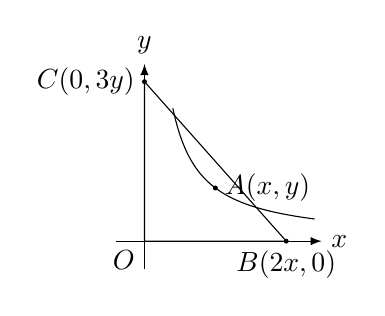
\begin{tikzpicture}[scale=0.45,>=latex]
  \draw[->] (-0.8,0)--(5,0) node[right]{$x$};
  \draw[->] (0,-0.8)--(0,5) node[above]{$y$};
  \node[below left] at (0,0){$O$};
  \draw[smooth,domain=0.8:4.8,samples=80] plot(\x,{3/\x});
  \coordinate (A) at (2,1.5);
  \coordinate (B) at (4,0);
  \coordinate (C) at (0,4.5);
  \draw (0,0)--(B)--(C)--cycle;
  \fill (A) circle(2pt) node[right]{$A(x,y)$};
  \fill (B) circle(2pt) node[below]{$B(2x,0)$};
  \fill (C) circle(2pt) node[left]{$C(0,3y)$};
\end{tikzpicture}
\end{center}

\end{eduProblemBlock}





\begin{eduAuxItem}{思路导航}
把底和高写成 $x,y$$\;\to\;$面积整理出 $xy$$\;\to\;$用 $xy=k$\end{eduAuxItem}




\begin{eduSubQuestionItem}{例题 4}
底和高用 $x,y$ 表示时，求 $k$。\end{eduSubQuestionItem}

\begin{eduDualExplain}
  \begin{eduExplainLeft}
    \eduColumnTitle{\eduIconBulb}{小贴士}
        \eduSideHint{最后一定回到 xy}{$B,C$ 不在反比例函数上，但 $A(x,y)$ 在图像上，所以 $xy=k$。}
  \end{eduExplainLeft}

  \begin{eduExplainRight}
    \eduColumnTitle{\eduIconBook}{解答}
      \eduExplainStep{1}{把底和高写成 $x,y$}{第一象限中 $x>0,y>0$，所以 $OB=2x$，$OC=3y$。}
      \eduExplainStep{2}{面积整理出 $xy$}{$S_{\triangle OBC}=\dfrac12\cdot2x\cdot3y=3xy$。}
      \eduExplainStep{3}{用 $xy=k$}{由 $3xy=24$ 且 $xy=k$，得 $3k=24$，所以 $k=8$。}
  \end{eduExplainRight}
\end{eduDualExplain}




\begin{eduSummaryBlock}{\eduIconPin}{方法提醒}
\begin{eduBulletList}
  \item 矩形面积：$|k|$。  \item 三角形面积：$|k|/2$。  \item 底高是 $x,y$ 的倍数时，先整理出 $xy$，再换成 $k$。  \item 最后检查象限或增减性。\end{eduBulletList}
\end{eduSummaryBlock}




\end{document}
